\begin{figure}[H]
\centering
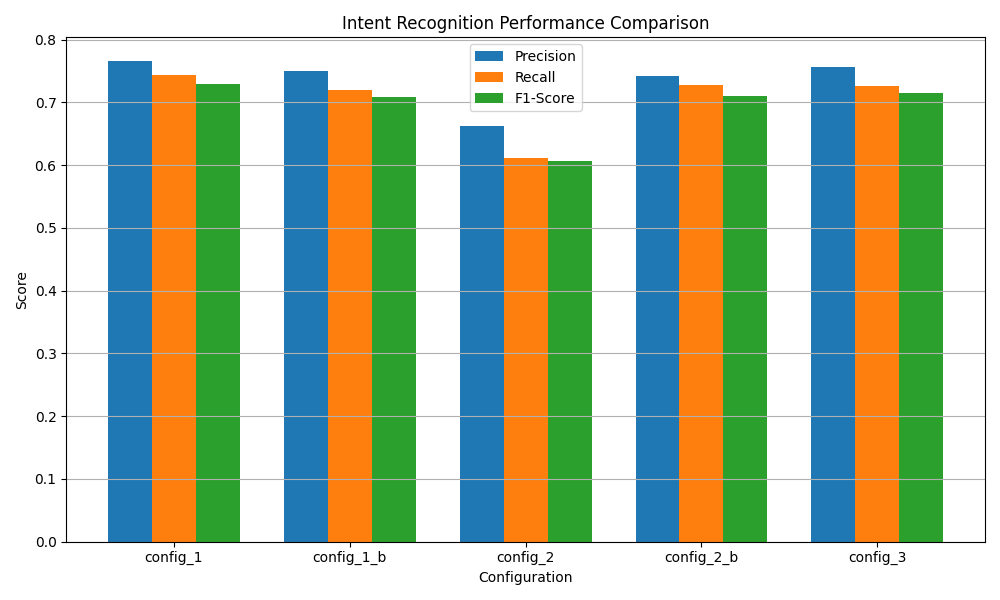
\includegraphics[width=8cm]{intent_comparison.png}
\caption{Intent recognition performance comparison across different configurations. The evaluation metrics include precision, recall, and F1-score using 5-fold cross-validation.}
\label{fig:intent_comparison}
\end{figure}

\begin{figure}[H]
\centering
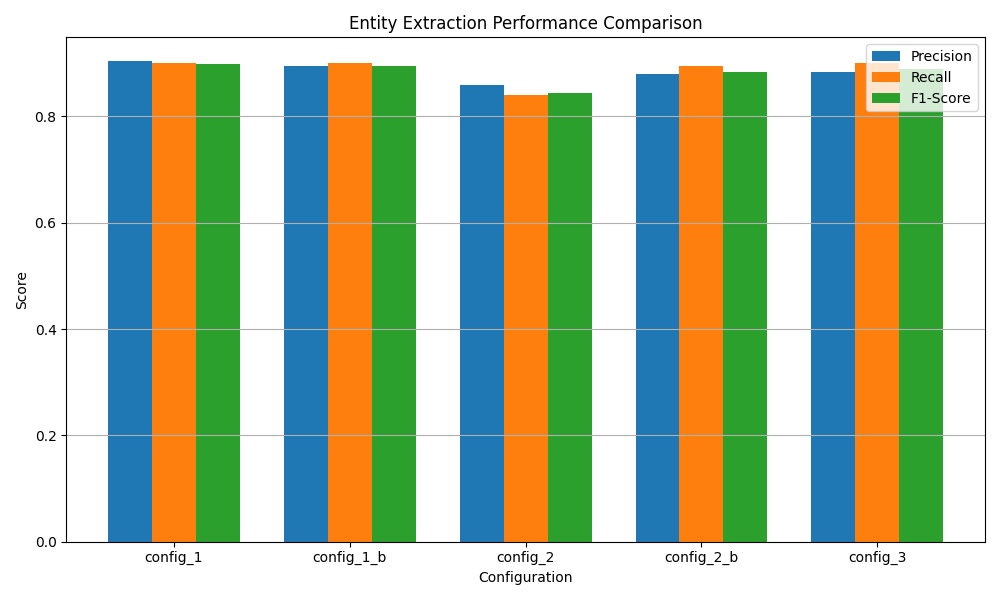
\includegraphics[width=8cm]{entity_comparison.png}
\caption{Entity extraction performance comparison across different configurations. The evaluation metrics include precision, recall, and F1-score using 5-fold cross-validation.}
\label{fig:entity_comparison}
\end{figure}

\begin{table}[H]
\caption{Performance metrics comparison across different model configurations. The table shows precision, recall, F1-score and support values, with Config\_3 achieving the highest performance across all metrics.}
\label{tab:performance_metrics}
\centering
\begin{tabular}{lcccc}
\toprule
\textbf{Configuration} & \textbf{Precision} & \textbf{Recall} & \textbf{F1-score} & \textbf{Support} \\
\midrule
Config\_3 & \textbf{0.709422} & \textbf{0.786223} & \textbf{0.733571} & 421.000000 \\
Config\_2\_b & 0.699327 & 0.776722 & 0.723040 & 421.000000 \\
Config\_1 & 0.667656 & 0.755344 & 0.695249 & 421.000000 \\
Config\_1\_b & 0.663895 & 0.738717 & 0.685669 & 421.000000 \\
Config\_2 & 0.610333 & 0.693587 & 0.636263 & 421.000000 \\
\bottomrule
\end{tabular}
\end{table}

\begin{table}[H]
\caption{Performance comparison of different model configurations on intent recognition and entity extraction tasks. The results show the average values across 5-fold cross-validation.}
\label{tab:performance_comparison}
\centering
\begin{tabular}{lcccccc}
\toprule
\multirow{2}{*}{\textbf{Configuration}} & \multicolumn{3}{c}{\textbf{Intent Recognition}} & \multicolumn{3}{c}{\textbf{Entity Extraction}} \\
\cmidrule(lr){2-4} \cmidrule(lr){5-7}
 & \textbf{Precision} & \textbf{Recall} & \textbf{F1-score} & \textbf{Precision} & \textbf{Recall} & \textbf{F1-score} \\
\midrule
Config\_1 & 0.765 & 0.754 & 0.739 & 0.904 & 0.899 & 0.898 \\
Config\_1\_b & 0.749 & 0.732 & 0.723 & 0.893 & 0.905 & 0.895 \\
Config\_2 & 0.662 & 0.621 & 0.607 & 0.859 & 0.840 & 0.845 \\
Config\_2\_b & 0.717 & 0.689 & 0.675 & 0.883 & 0.871 & 0.873 \\
Config\_3 & \textbf{0.768} & \textbf{0.766} & \textbf{0.755} & \textbf{0.918} & \textbf{0.921} & \textbf{0.919} \\
\bottomrule
\end{tabular}
\end{table}

\begin{table}[H]
\caption{Dialogue evaluation process examples with translations.}
\label{tab:dialogue-eval}
\footnotesize
\setlength{\tabcolsep}{4pt}
\begin{tabular}{p{0.18\textwidth}p{0.37\textwidth}p{0.37\textwidth}}
\toprule
\textbf{Evaluation Step} & \textbf{Example (Congolese Swahili)} & \textbf{Translation (English)} \\
\midrule
\multicolumn{3}{l}{\textbf{Example 1}} \\
\midrule
\textbf{User Turn} & Kambi za wakimbizi wapi? & Where are the refugee camps? \\
\textbf{Bot Turn} & \begin{minipage}[t]{0.37\textwidth}
RUSAYO 2 (Rutshuru) - Uwezo: 2280\\
KASHUGA (Rutshuru) - Uwezo: 10976\\
MATER DEI (Rutshuru) - Uwezo: 460\\
MPATI (Rutshuru) - Uwezo: 10976
\end{minipage} & 
\begin{minipage}[t]{0.37\textwidth}
RUSAYO 2 (Rutshuru) - Capacity: 2280\\
KASHUGA (Rutshuru) - Capacity: 10976\\
MATER DEI (Rutshuru) - Capacity: 460\\
MPATI (Rutshuru) - Capacity: 10976
\end{minipage} \\
\textbf{Task Identification} & \begin{minipage}[t]{0.37\textwidth}
1. Kujibu swali\\
2. Kutoa maelezo ya kitu\\
3. Kutoa orodha ya vitu
\end{minipage} & 
\begin{minipage}[t]{0.37\textwidth}
1. Answer query\\
2. Provide entity details\\
3. List entities
\end{minipage} \\
\textbf{Task Success} & Yote yalifanikiwa (y/y/y) & All tasks were successful (y/y/y) \\
\textbf{Error Type} & 0 - Hakuna kosa (No error) & 0 - No error \\
\midrule
\multicolumn{3}{l}{\textbf{Example 2}} \\
\midrule
\textbf{User Turn} & Naeza pata wapi chakula cha msaada? & Where can I get food aid? \\
\textbf{Bot Turn} & PAM inapena chakula ya msaada kila wiki Kitchanga na Mweso. & WFP gives food aid every week in Kitchanga and Mweso. \\
\textbf{Task Identification} & \begin{minipage}[t]{0.37\textwidth}
1. Kujibu swali\\
2. Kuelekeza eneo\\
3. Kutaja shirika
\end{minipage} & 
\begin{minipage}[t]{0.37\textwidth}
1. Answer query\\
2. Provide entity details\\
3. List entities
\end{minipage} \\
\textbf{Task Success} & Yote yalifanikiwa (y/y/y) & All tasks were successful (y/y/y) \\
\textbf{Error Type} & 0 - Hakuna kosa (No error) & 0 - No error \\
\bottomrule
\end{tabular}
\end{table}

{\footnotesize
\begin{algorithm}[H]
\DontPrintSemicolon
\SetAlgoLined
\caption{Dialogue Evaluation Procedure}\label{algo:dialogueeval}
\SetKwInOut{Input}{Input}\SetKwInOut{Output}{Output}
\Input{Dialogue with alternating User and Bot turns}
\Output{Annotated dialogue with task types, success status, error types}

\ForEach{(UserTurn, BotTurn) in Dialogue}{
    \tcp{Step 1: Identify tasks in BotTurn}
    Classify each task as: (1) Provide Information (2) Answer Query (3) Provide Entity Details (4) List Entities (5) Explain Relationship (6) Other\;
    \ForEach{Task in BotTurn}{
        Record task type and success status (Yes/No)\;
    }
    \tcp{Step 2: Record error type}
    Mark error as: (0) None (1) Substitution (2) Deletion (3) Insertion\;
}
\tcp{Step 3: Suggest corrections}
\ForEach{BotTurn in Dialogue}{
    If correction needed, annotator writes ideal response\;
}
Store all annotations for the dialogue\;
\end{algorithm}
}
\normalsize 

\acknowledgments{The authors would like to express their sincere gratitude to Honore Mbaya for his invaluable assistance in verification of the Congolese Swahili language resources. His expertise in local dialects and humanitarian contexts significantly enhanced the quality and authenticity of our dataset. We also acknowledge the community radio stations and local NGOs that provided access to emergency call data critical for this research.

In this section you can acknowledge any support given which is not covered by the author contribution or funding sections. This may include administrative and technical support, or donations in kind (e.g., materials used for experiments). Where GenAI has been used for purposes such as generating text, data, or graphics, or for study design, data collection, analysis, or interpretation of data, please add "During the preparation of this manuscript/study, the author(s) used [tool name, version information] for the purposes of [description of use]. The authors have reviewed and edited the output and take full responsibility for the content of this publication."} 